% !TEX root = ../Survey.tex
In this section we describe  various algorithmic techniques that are either folklore, used in several papers,  or ones that  originate from papers not covered by the survey.
The purpose of the  section is to outline  a common toolbox useful for labeling schemes and to point out the similarity between some of the techniques. 

\subsection{Binary strings and bit tricks} \label{section:Misc-Tools}
\subsubsection{Number representation}
Labels  and words can be seen both as integers or as  boolean strings. \todo{It's not completely clear to me what ``words'' are, nor is it clear how a label can be seen as an integer?}
In order to represent any possible number in the range $\{1 \dots n\}$, $\lceil \log n \rceil$ bits are required.
Therefore, the number of bits in  a binary string $\bin(x)$ is $\lceil \log x \rceil$, and we occasionally denote it by $ \vert \bin(x) \vert$. \todo{Would it not be better to consider $\{0,\dots ,n-1\}$ and use $\fl{\log x}$ bits?}

A method  used in \emph{all} papers surveyed   is the concatenation of  meaningful bits.
Given two strings $\alpha$ and $\beta$, we denote the concatenated string  $\alpha \circ \beta$.
Both $\alpha$ and $\beta$ may be extracted  from the string $\alpha \circ \beta$  by a na\"ive  \emph{separating} string.
 A \emph{separating string} is a string of $m= \vert \alpha \vert + \vert \beta \vert$ bits with $'1'$ in bit number $\vert \alpha \vert$ and $'0'$ in the rest.
A  label with $m$ bits of two or more parts, each of variable size, may be described as a corresponding label of size $2m$, such that each part can be extracted from it using the added separating string.
When we are interested in reducing $2m$ further, and have a fixed number of parts  $c$, we may use a label of size $m+ c \log m$.
\todo{This requires that we know the length of the string. Can we always assume that? (In some situations with a ``data stream'', we know when the string starts but not necessarily when it ends.)}
Moreover, suppose we have  a label containing two parts  $\alpha$ and $\beta$, then we may extract both parts using an improved separating string with  $\log \min(\vert a \vert ,\vert b \vert)$  bits.
It follows that any constant number of bits attached to a string does not change its size asymptotically. 
Most labeling schemes reviewed utilise this property to attach a constant number of bits to be   used later by the decoder.

	\subsubsection{Padding}\label{tec:padding}
	The following bit-trick allows for parts of a label to consistently have the same size by adding a single bit to the largest resulting label.
	Suppose we want to represent $x$ where  $\vert \bin(x) \vert < \log n$, then we can use \textit{exactly} $\log n +1$ bits to describe $x$ using the bit string $\bin(x) \circ 1 \circ 0^i$ where $i=n+1 - \vert \bin(x) \vert$, and  $0^i$ is the binary string composed of $i$ times $0$.
		
	\subsubsection{Approximation using $O(\log\log n)$ bits}\label{tec:approx}
	 Let $k \in  \{1 \dots n\}$ be an integer, and recall that  $\bin(k)$ requires at most $\lceil \log n \rceil$ bits. Using $\lceil \log \log n \rceil$ bits we can represent a number $k'$ such that $\ceil{k/2} < 2^{k'} \leq k$ or, alternatively such that $k \leq 2^{k'} < 2k$.
	We  set  $k' =  k[p]$,  where $k[p]$ is the position of the most significant bit set to $'1'$ in $\bin(k)$.
	 Now $\bin(k')$ is interpreted as a $1/2$-approximation of $k$  by computing the appropriate  binary string $1 \circ 0^{k'-1}$. \todo{This definition of ``approximation'' does not comply with the previous one}
	Similarly, we can produce a $2$-approximation of $k$ by  the  binary string $1 \circ 1^{k'-1}$.
	Any additional bit stored in $k'$ now increases the accuracy of the approximation by a factor of two.
	The latter is in particular useful since by storing  additional  $\ceil{ \log \log n }$ bits we can represent a number $k^*$ such that $k \leq k^* < \floor{(1+1/ \log n)k}$, respectively~$\floor{\frac{\log n}{\log n+1}k} < k^* \leq k$.

\subsubsection{Word storing in a string}\label{tec:wordinside}
	We conclude this section with the following  bit-trick, which is based on the following facts.
	For any two integers $j$ and $k$, the value of the bit string $\bin(j) \circ \bin(k)$ is $j \cdot 2^{\vert\bin(k)\vert}+k$, and in addition $j<2^{\vert \bin(j)\vert}$.
			\begin{lemma} \label{lemma:numberinside}
			Let $w$ and $z$ be two integers. One can compute  an integer $x \in [z,z+2^{ \vert \bin(w) \vert} )$ such that $\bin(w)$ is a suffix of $\bin(x)$.
			\end{lemma}
			\begin{proof}
			 We  compute $d = \floor{z/ 2^{\vert \bin(w) \vert}}$ and denote the difference $m = z-d$.
			 Consider now the number $x$ represented by the bit-string $ \bin(d) \circ \bin(w)$.
			 If $w \geq m$  then $x \geq z$ and also   $x=z-m+w \leq z+w < z + 2^{\vert  \bin(w) \vert}$. \todo{I think something is wrong here. Why is $x=z-m+w$?}
			 If $w < m$ then $x$ may be smaller than $z$. 
			 We therefore increase the value of  $x$ by  $2^{\vert \bin(w) \vert}$, represented by  $\bin(d+1) \circ \bin(w)$.	
			 Now, $x = z- m + 2^{\vert  \bin(w) \vert}  + w > z + w \geq z$ since $m< 2^{\vert \bin(w) \vert}$, and also $z-m+ 2^{\vert \bin(w) \vert} +w < z +  2^{\vert \bin(w) \vert}$ since $w<z$. 
			 \end{proof}
			
\subsection{Efficient encodings}\label{sec:efficient-encoding}
\subsubsection{ Depth-first traversal}\label{tec:dfs}
We denote a depth-first traversal of a tree by $\dfs$.
A substantial number of the results surveyed use  a node numbering  by a  particular depth first traversal of a tree.
A depth-first traversal of the tree is denoted $\dfsi$ if  children of small size\footnote{The \emph{size} of a node in a tree is the number of its descendants.} are visited before children of larger size. \todo{This seems like an unfortunate notation. The ``$i$'' is normally used for indexing.}
Given a tree $T=(V,E)$  every node $v \in V$ receives the number $\dfsi(v)$ from $\dfsi$, and we occasionally refer to it as the $\dfsi$ identifier of $v$.


\subsubsection{Suffix-free codes}\label{tec:suffix}
A \emph{code} is a set of words,\todo{....and what is a word?} and a code is \emph{suffix-free}\footnote{ suffix-free codes are also known as suffix codes.}, if no word in the code is the suffix of another word.
As a concrete example consider the following collection of words:
$code_0(x) = 1 \circ 0^x$, where $0^x$ is the binary string composed of $x$ times $0$.
This suffix-free code is inefficient since the number of bits required to store $code_0(x)$ is $2^{\vert \bin(x) \vert}+1$.
We can  extended this code  to an efficient  recursively constructed suffix-free code by
$code_{i+1}(x) = \bin(x) \circ code_i(\vert bin (x) \vert - 1)$ for every $i \geq 0$. 
For example,  $code_0(8) = 100000000$, $code_1(8) = 1000 1000$, $code_2(8) = 1000 11 10$.  
In order to store  $code_1(x)$ and $code_2(x)$ we use $2 \floor{\log{x}} +2$ and $\floor{\log x}+ 2\floor{\log \log x}+ 3$ bits respectively.
The method can be applied recursively  up to $\log^* x $ times such that the length of 
 $code_i(x)$  is at most $   \floor{\log x}  + \floor{ \log  \log x} + \dots +  O(\log^* x)$\footnote{$\log^*$ is the number of times $\log$ should be iterated before the result is at most $1$.}.
 
Suffix-free codes are useful for labeling schemes for one important property: a concatenation of suffix codes is by itself a suffix code. For labels constructed by two or more parts of variable sizes, suffix codes allow for an encoding of those parts.
It is worth noting that, by Kraft's inequality~\cite{cover2012elements}, no  uniquely decipherable encoding  for boolean string $s$ can enjoy a size of less than $s + \log  s$, for a  sufficiently large $s$.

\subsubsection{Alphabetic sequences}\label{tec:alphabetic}
The following Lemma is useful to assign labels to the nodes of a rooted path that achieves the following two properties:
First, nodes of  a large size are assigned a small label, and  second, the labels maintain a total order among the path's nodes.

Let $\lex$ denote the lexicographical order of binary strings. A finite sequence $(a_i)$ of nonempty, binary strings $a_i\in\{\zero,\one\}^*$ is \emph{alphabetic} if $a_i \lex a_j$ for $i<j$. 


\begin{lemma}\label{lemma:Gilbert}
Given a finite sequence $(w_i)$ of positive numbers with $w=\sum_iw_i$, there exists an alphabetic sequence $(a_i)$ with $|a_i|\leq \floor{\log w - \log w_i}+1$ for all $i$.
\end{lemma}	
\begin{proof}
The proof is by induction on the number of elements in the sequence $(w_i)$. If there is only one element, $w_1$, then we can set $a_1=0$, which satisfies $|a_1|=1 =\floor{\log w_1-\log w_1}+1$.  Suppose that there is more than one element in the sequence and that the theorem holds for shorter sequences. Let $k$ be the smallest index such that $\sum_{i\leq k} w_i>w/2$, and set $a_k=0$.  Then $a_k$ clearly satisfies the condition. The subsequences $(w_i)_{i<k}$ and $(w_i)_{i>k}$ are shorter and satisfy $\sum_{i<k}w_i\leq w/2$ and $\sum_{i>k}w_i\leq w/2$, so by induction there exist alphabetic sequences $(b_i)_{i<k}$ and $(b_i)_{i>k}$ with $|b_i|\leq \floor{\log(w/2)-\log w_i} +1 = \floor{\log w-\log w_i} $ for all $i\neq k$. Now, define $a_i$ for $i<k$ by $a_i=0\circ b_i$ and for $i>k$ by $a_i=1\circ b_i$. Then $(a_i)$ is an alphabetic sequence with $|a_i|\leq\floor{\log w-\log w_i}+1$ for all $i$.
\end{proof}

Viewed differently,  alphabetic sequence are possible since each number $w_j$  ($1 \leq j \leq i$) can be represented by a number between  $\sum_{i=1}^{j-1}w_i$ and  $ \sum_{i=1}^{j-1}w_i +2^{\lfloor \log w_j \rfloor}$  with at least $\lfloor \log w_j \rfloor$ $0$s in its least significant bits that can be discarded.
As an example, the sequence $(w_i)=(2,8,1,1,4)$ with $w=16$,    may be represented by $0000,1000,1010,1100,1110$ and, accordingly, $(a_i) = (0,1,101,11,111)$.
Numbers in $(a_i)$ now have a total order with respect to the order in which they were in $(w_i)$. Given two numbers, a decoder may equalise their size by adding zeros to the number with less digits. \todo{What does this last sentence have to do with all the rest?}



\subsection{Tree decompositions}\label{section:Tree-decompositions}
This section is dedicated to recursive tree decomposition techniques that were found useful in  the results surveyed.
The \emph{heavy-light} and \emph{separator} are two well known techniques, and in this section we expose their similarity.
The \emph{splines} decomposition can be seen as an extension and generalisation of \emph{heavy-light} decomposition.
The \emph{clustering} decomposition was only used once in the surveyed literature but has potential for further use. \todo{That seems a bit subjective. Do we want to niclude it?}
Some of the techniques create a  \emph{path-decomposition} of a tree $T$, which is a collection of paths in $T$ such that every node $v \in T$ is a member of exactly one path.


\subsubsection{Heavy-light decomposition}\label{tec:heavylight}
\citeN{hareltarjan} show how to create a path-decomposition of a rooted tree where each node of a path, except its top-node\footnote{The top-node of a path in a tree $T$ rooted in $r$ is the node closest to $r$.}, has maximum size among its siblings. 
The decomposition allows the location of a node in the tree to be described by the sequence of paths that must be traversed in order to reach the node from the root. 

Let $T$ be a tree with root $r$. The nodes of $T$ are classified as either \emph{heavy} or \emph{light} as follows. The root is light. For each internal node $v\in T$, pick one child $w$ whose size is maximal among the children of $v$ and classify it as heavy; classify the other children of $v$ as light.  We denote the unique heavy child of $v$ by $\hchild(v)$ and the set of light children of $v$ by $\lchildren(v)$. The \emph{light size} of a node $v$ is the number 

$$ \lsize(v) =  1+\sum_{\mathclap{u\in \lchildren(v)}} \size(u).$$

Note that if $v$ is a leaf or has only a single child then
$\lsize(v)=1$, and if $v$ is internal then 
$\lsize(v)=\vert v \vert - \vert \hchild(v) \vert$.

An edge connecting a light node to its parent is a \emph{light edge}, and an edge connecting a heavy node to its parent is a \emph{heavy edge}. By removing the light edges, $T$ is divided into a collection of \emph{heavy paths}. The set of nodes on the same heavy path as $v$ is denoted $\hpath(v)$.  See Figure~\ref{fig:heavylighttree} for an example.
\begin{figure}
\centering

\begin{tikzpicture}[scale =0.7,inner sep=0pt, minimum size=1ex, sibling distance=2em]
\tikzstyle{every node}=[draw,circle]
\Tree  [ 
.{} %.{}
	\edge[dashed]; [.{} [.\node[fill=black]{}; \edge[dashed]; [.{} \node[fill=black]{}; ]
							       [.\node[fill=black]{}; \node[fill=black]{}; \edge[dashed]; {} ]
                       					       \edge[dashed]; [.{} \node[fill=black]{}; ]
					    ] 
					    \edge[dashed]; {} ]
	\edge[dashed];  [.{} \node[fill=black]{}; ]
	[.\node[fill=black]{}; \edge[dashed]; {}
			[.\node[fill=black]{}; \edge[dashed]; {}
					[.\node[fill=black]{}; \edge[dashed]; {}
							\node[fill=black]{};
							\edge[dashed]; {} ]
					\edge[dashed]; {} ]
			\edge[dashed]; {} ]
	]
\end{tikzpicture}
\caption{
A tree in which light and heavy nodes have been marked with ``$\circ$'' and ``$\bullet$'', respectively, and heavy and light edges have been drawn with solid and dashed lines, respectively.} \label{fig:heavylighttree}
\end{figure}

Given a node $v$ in $T$, consider the list of light nodes $u_0 \dots u_k$ encountered on the path from the root $r$ to $v$. The first of these light nodes is the root, $r=u_0$, and we denote the list  $u_0 \dots u_k$ as  $\lpath(v)$. The number $k$ is the \emph{light depth} of $v$, denoted $\ldepth(v)$. The light depth of $T$, $\ldepth(T)$, is the maximum light depth among the nodes in $T$. Since the size of every light node is bounded by the size of its heavy sibling, the size of $u_{i+1}$ is at most half the size of $u_i$. From this, it follows that $\ldepth(v)\leq \floor{\log n}$ for all nodes $v$, where $n$ is the number of nodes in $T$. 

Note that the results surveyed which use this path-decomposition perform also a $\dfsi$ traversal of the tree (see Section~\ref{tec:dfs}).

\subsubsection{Separator}\label{tec:separator}
Two sets of nodes in a graph are separated if  no node in one is adjacent to any node in the other.
A separator is typically defined as a subset of nodes in a graph $G$ whose removal from $G$ separates the graph into two subsets $U$ and $V$
such that $\vert U \vert \leq \vert V \vert < 2 \vert U \vert$~\cite{chung1989separator}.
For all trees there exist a separator that consist of a single node.
\begin{theorem}~\cite{jordan1869assemblages}\label{thm:separatorexits}
Given a tree $T$ rooted in node $r$, we can find, in linear time,  a single node whose removal  separates  $T$ into  subtrees of at most $n/2$ nodes each.
\end{theorem}
\begin{proof}
Consider any node $v \in T$. If $v$ does not divide $T$ into components of size at most $n/2$ each, then $v$ has a neighbour $u$ in a subtree of size more than $n/2$.
 Move into the  subtree rooted by $u$  and recurse. This process will never traverse the same edge twice, thus, the separator is found in at  most $n$ steps.
\end{proof}
The result also holds naturally for forests. ~\citeN{korman2007compact} use Theorem~\ref{thm:separatorexits}  to define a \emph{separator tree} described briefly hereafter.
Given a tree $T=(V,E) \in Trees(n)$ we construct a \emph{separator tree} denoted $T^{sep}$ in the following manner.
The root $r$  of $T^{sep}$ is the separator, its children are the separators of the subtrees  described in  Theorem~\ref{thm:separatorexits} for $r$. The subtree rooted by each of those children is defined recursively in the same manner. The depth of the corresponding separator tree $T^{sep}$ is $\log n$. 
A  node $v \in V$  on the path $r \leadsto v$ in $T^{sep}$ with depth $i$ ($0 \leq i \leq \log n -1$)  has now some interesting properties. 
First, it is a separator for a subtree in $T$  of size at most $2^{\log n- i}$, in which both $v$ and  all its children in $T^{sep}$  are present. 
Second, $v$ is a node in  all of the  subtrees associated with  $v$'s ancestors in $T^{sep}$. 
For a demonstration, see Figure~\ref{fig:separator}.

				\begin{figure}[!ht]
				\centering
				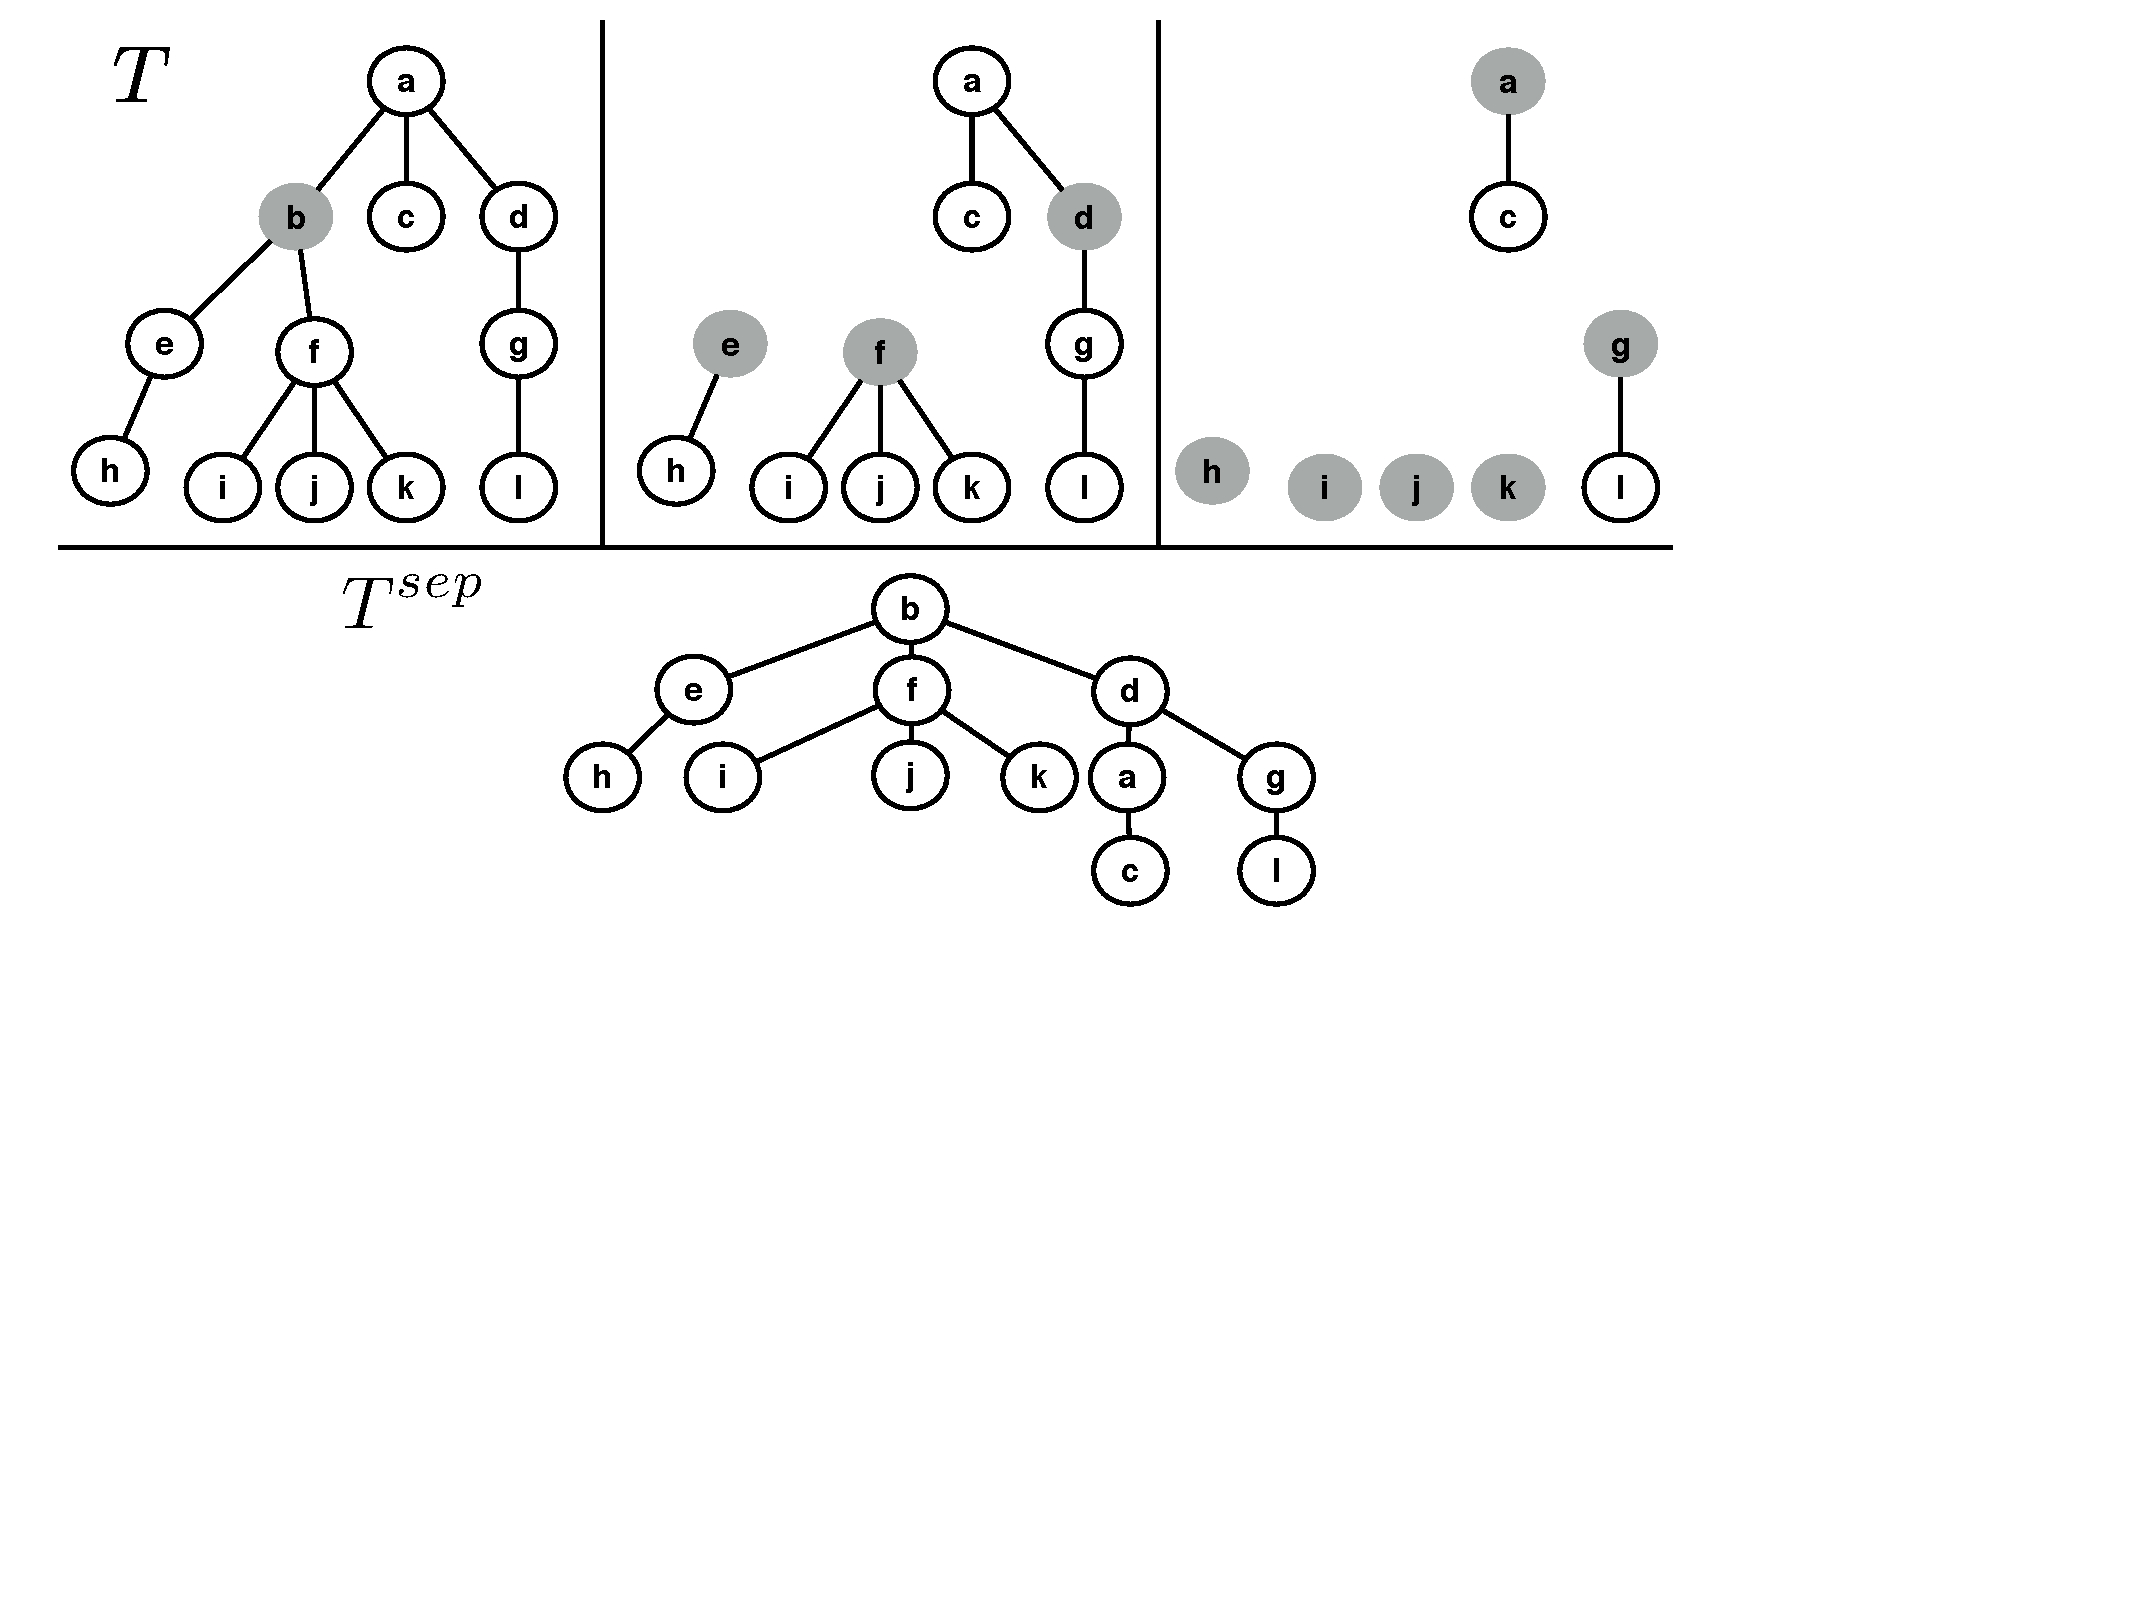
\includegraphics[width=80mm]{./Figures/Separator.pdf}
				\caption{Separator tree  for  the tree  $T$, with separator nodes marked  in grey. Top row:  $T$ rooted at $a$ (left). The forest resulted by removing the separator $b$ from  $T$ (center).  The remaining  forest after removing the  separators $e,f,d$ (right). Bottom row: the resulting $T^{sep}$. }
				\label{fig:separator}
			\end{figure}
			

 
\subsubsection{Spines decomposition}\label{tec:Splines}
This path-decomposition was invented by \citeN{Thorup01}, and used by \citeN{Korman10}.
Similarly to heavy-light decomposition, a \emph{spines decomposition}  decomposes an $n$ node tree $T$  into  a collection of paths, using an additional parameter, an integer $1 \leq b \leq n$.
A node $v$ is $heavy_{s}$ if $size(v) \geq n/b$ and $light_{s}$ otherwise. \todo{Is this standard terminology? It seems a bit weird to me...}
Note that the heavy nodes in $T$ induce a subtree rooted by the root of $T$, which is always  a $heavy_{s}$ node.
$T_h$ is the subtree of $T$ which spans the heavy nodes, and we note that  $T_h$ has at most $b$ leaves.
We  create a path-decomposition of $T_h$  by removing  every edge $(u,v)$ where $u$ has more than one child in $T_h$.
 This results in at most  $2b-1$ paths  $P_1 \dots P_l$, ($1 \leq l \leq 2b-1$) which  we denote as  $heavy_{s}$ paths (some of which may consist of a single node). When $b=2$, the  single $heavy_{s}$  path is referred  to  as the \emph{ spine} of $T$.

The spines decomposition of $T$ is  constructed recursively for subtrees in the forest $T \setminus T_h$ by using the above path-decomposition. 
The removal of $T_h$ from $T$ results in a forest $F$.
Note that a $light_{s}$ node $v$ in $T$ adjacent to a node in $T_h$ is  a root of a tree $T_v \in F$ of size $\size(v) \leq n/b$.
The decomposition stops when all nodes in $T$ are  $heavy_{s}$ nodes at some recursive step, and both node and path are of  \emph{level} $i$ if they occur at step $i$ in the decomposition.
Using  arguments similar to those for heavy-light decomposition, it follows that within at most $\log_{b} n$  steps all nodes in $T$ are $heavy_{s}$ nodes. 
See Figure~\ref{fig:ladder} for a demonstration.

				\begin{figure}[!ht]
				\centering
				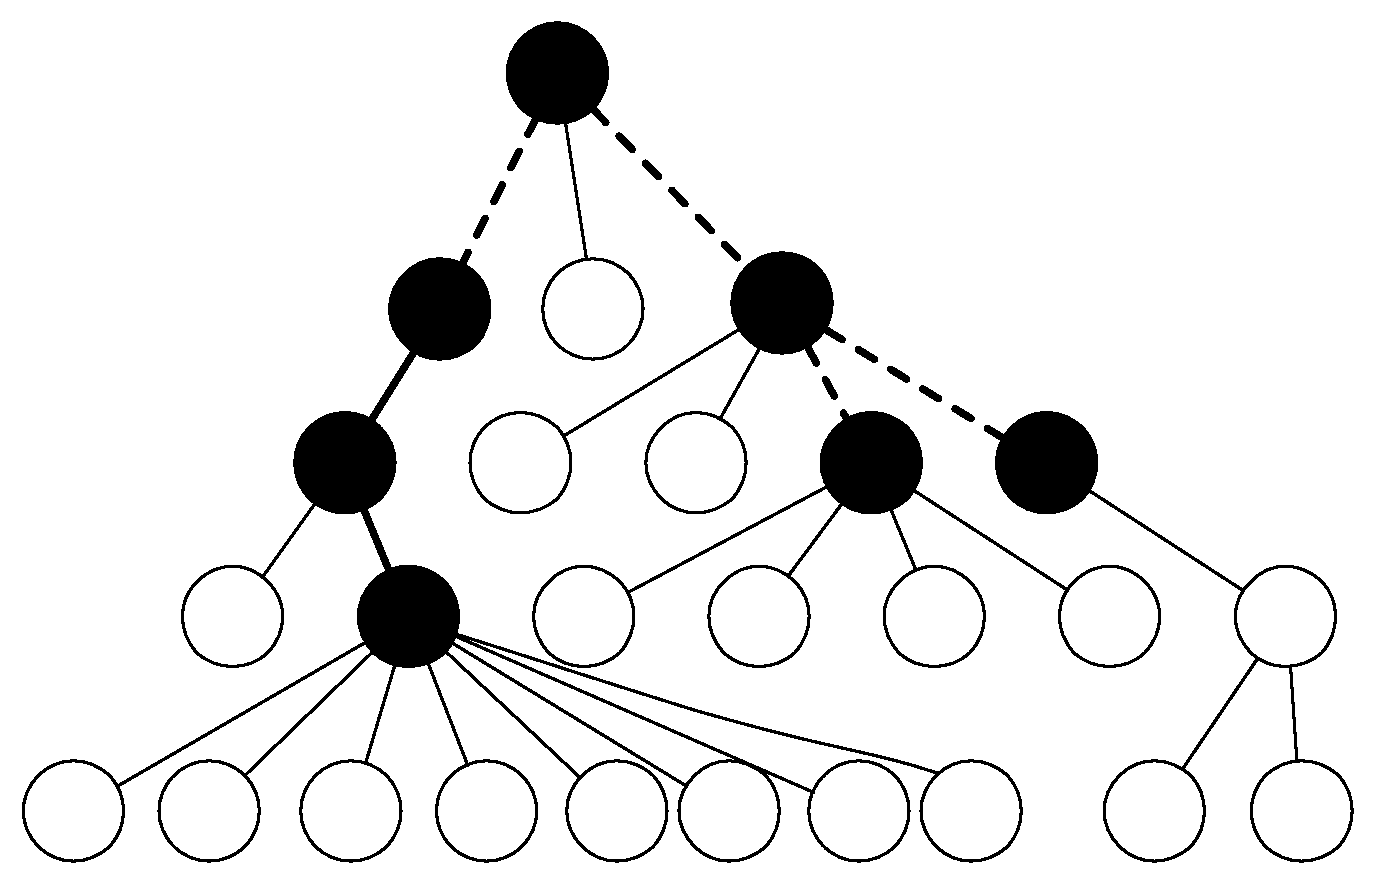
\includegraphics[width=50mm]{./Figures/Ladder_decomp.pdf}
				\caption{The first step of a  spines decomposition  of $T$ with $b=6$ for a tree with $n=24$ nodes. Black nodes are $heavy_s$ nodes, and the rest are $light_s$ nodes for the first step. Hatched lines are removed from $T_h$  and the emphasised edges mark the $heavy_s$ paths.}
				\label{fig:ladder}
			\end{figure}
			 

\subsubsection{Clustering}\label{tec:clustering}
The following  definitions are used to prove  that, given a number $x$ between $1$ and $n$, every tree can be decomposed into at most $n/x$ clusters with $O(x)$ nodes each, such that every cluster has at most two nodes in common with other clusters.

\begin{definition} \label{dfn:cluster}
Let $T$ be a tree of size $n = \vert V(T) \vert >1$.
 For a connected subtree $C$ of $T$, we call a node in $V(C)$ incident with a node in $V(T) \setminus V(C)$ a \emph{boundary node}.
The boundary nodes of $C$ are denoted by $\delta C$. 
A \emph{cluster} is a connected subtree of $T$ where $\vert \delta C \vert \leq 2$.
We denote $C(u,v)$ a cluster with the boundary nodes $u$ and $v$, where $depth(u)< depth(v)$.
If a cluster has only one boundary node, we associate  its rightmost leaf\footnote{The rightmost leaf of a tree $T$ is the last leaf encountered in the $\dfs$ traversal (see Section~\ref{tec:dfs}) of $T$.}  as the second boundary node.
Such clusters are called \emph{leaf} clusters. The remaining clusters are called \emph{internal} clusters.
 A set of clusters $\cs$ is a \emph{cluster partition} of a tree $T$ with root $r$ if and only if $V(T) = \cup_{C \in \cs}V(C)$, $E(T)= \cup_{C \in \cs} E(C) $, and for any distinct $C_1,C_2 \in \cs$, $E(C_1) \cap E(C_2) = \emptyset$, $\vert E(C_1) \vert \geq 1$, and $ r \in V(C)$ if $r \in \delta C$. \todo{The latter is unclear to me: doesn't this always hold for all nodes by definintion?}
\end{definition}

				\begin{figure}[!ht]
				\centering
				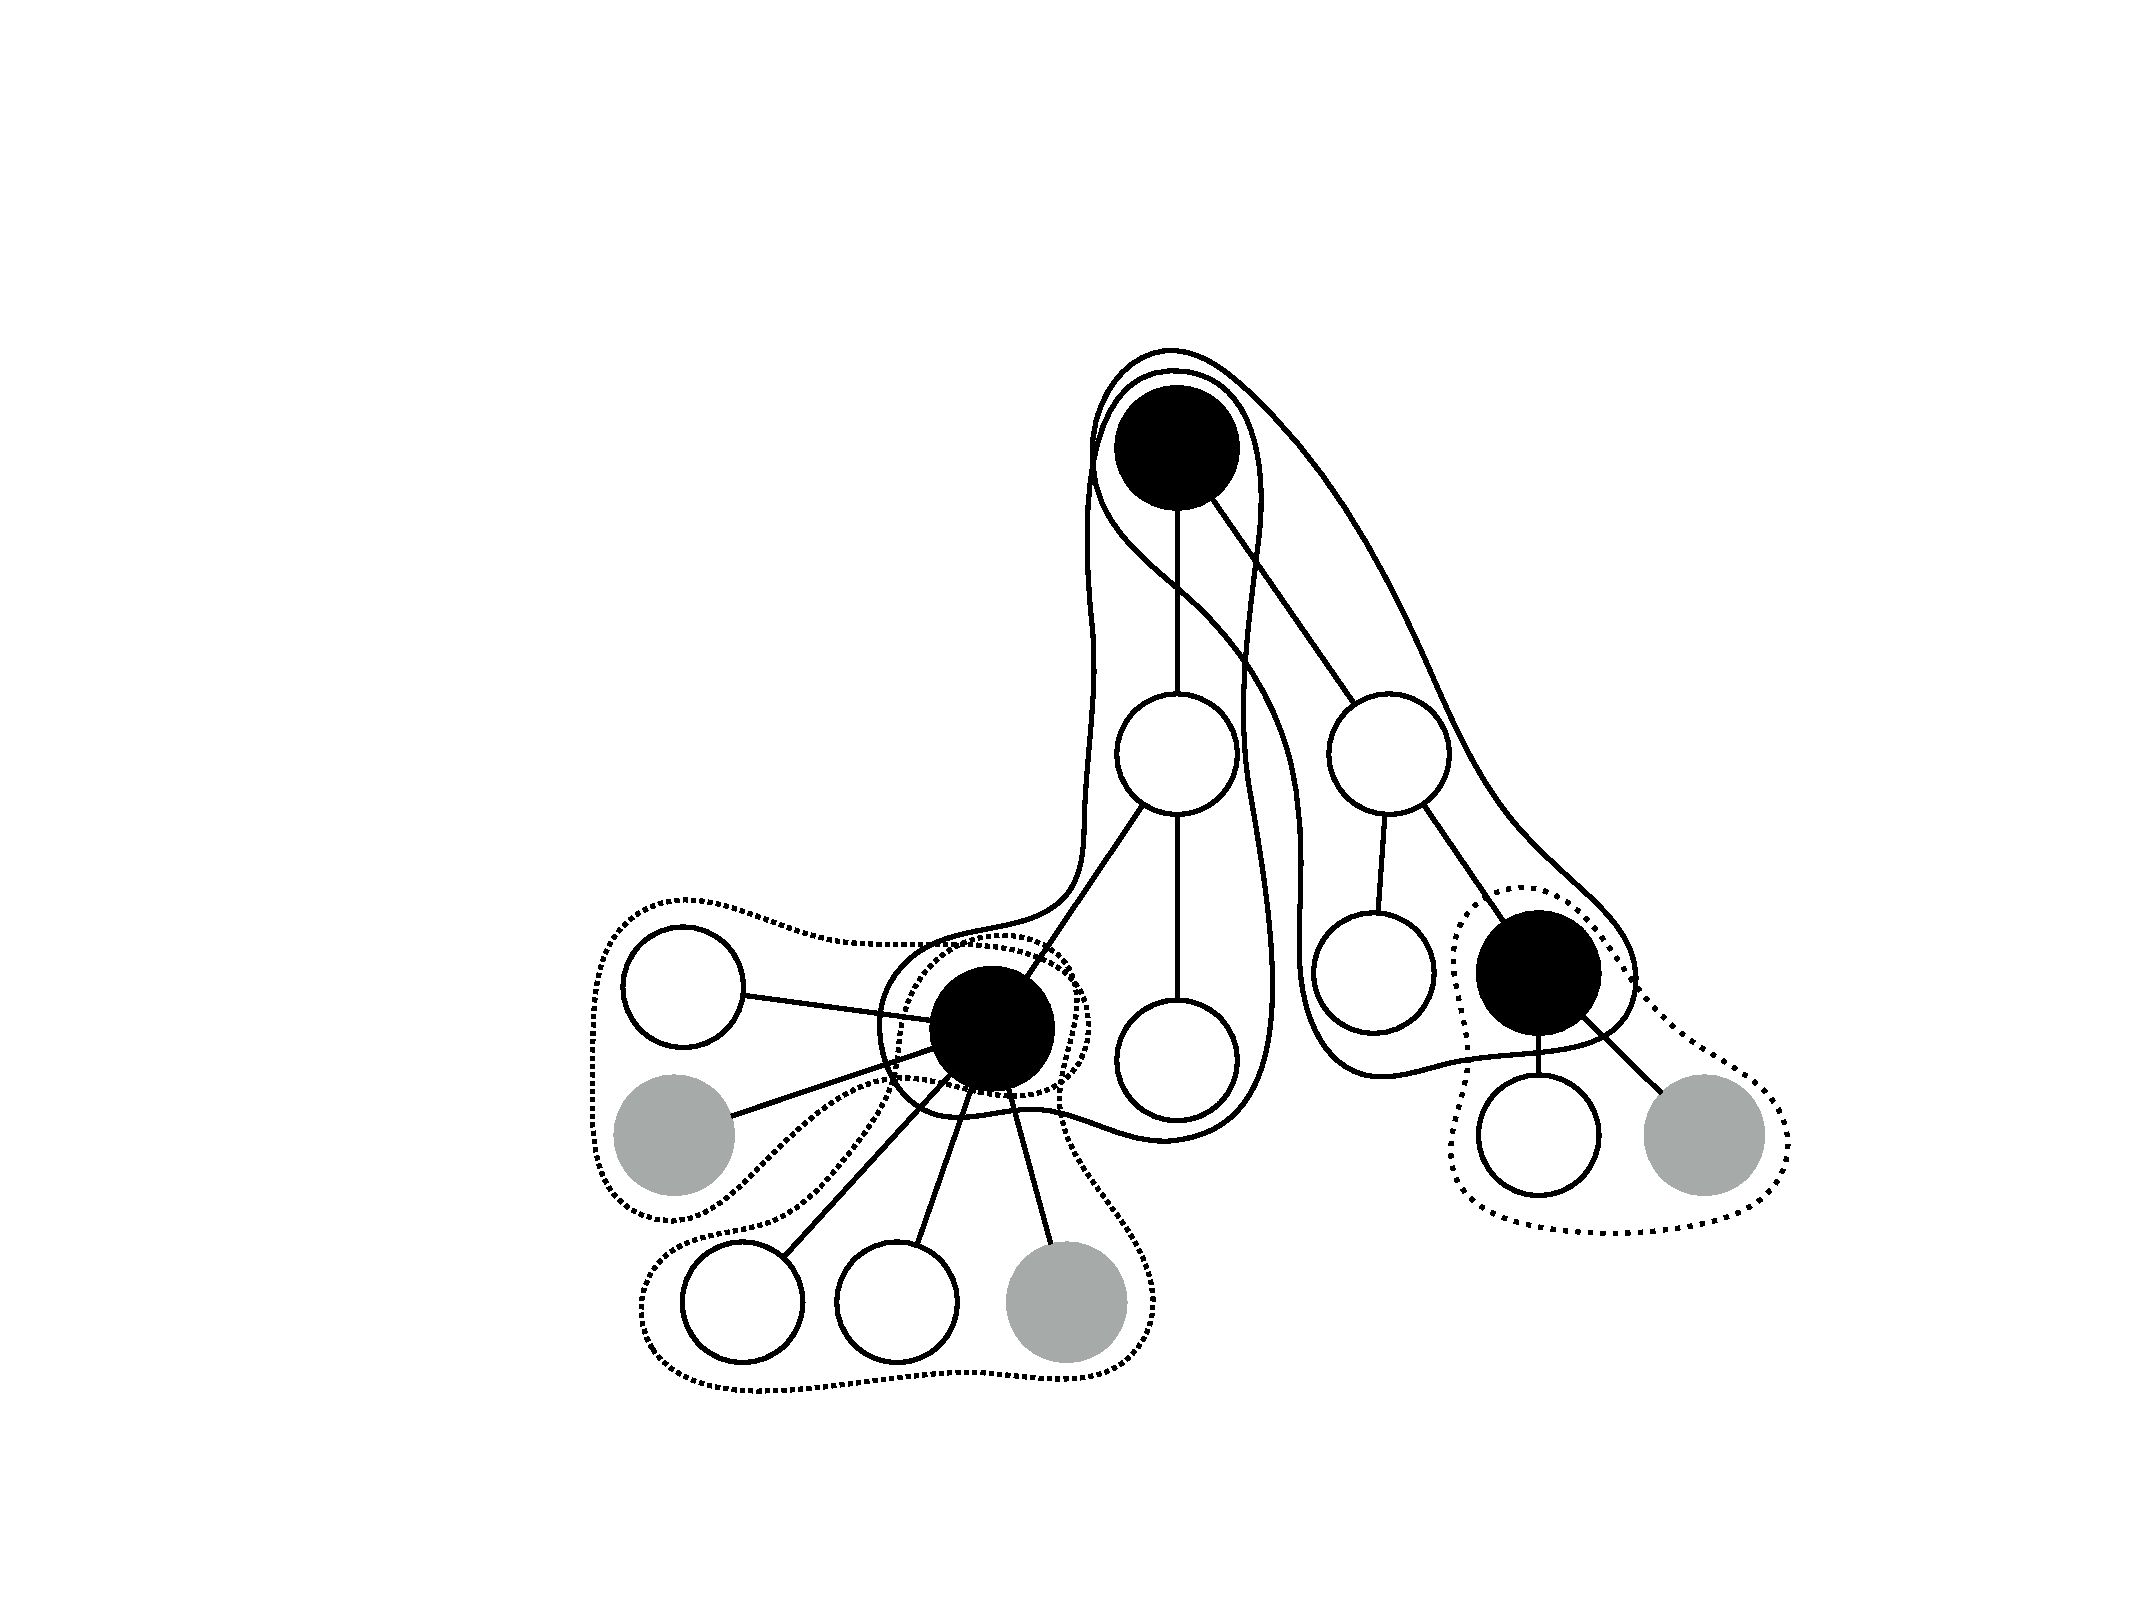
\includegraphics[width=40mm]{./Figures/newclustering.pdf}
				\caption{A demonstration of a nice cluster partition with $n=14$ and $x=4$. The dotted clusters are leaf clusters and the rest are internal clusters. The black nodes are boundary nodes, and the grey nodes  are the second boundary nodes added.}
				\label{fig:niceClusterDemo}
			\end{figure}
			
\begin{definition}\label{dfn:nice-cluster-partition}
Given a tree $T$ with $n>1$ nodes rooted at $r$ and a parameter $ 1 \leq x \leq n$. A cluster partition $\cs$ is a \emph{nice cluster partition}  if   $\vert \cs \vert \leq n/x$  and  $\vert V(C) \vert \leq cx$ for all $C \in \cs$, for some constant $c$. 
\todo{Shouldn't this definition depend on x? As in ``x-nice''?}
\end{definition}


\begin{lemma}\label{lemma:decomposition}
For any tree $T$ with $n$ nodes and any  $1 \leq x \leq n$ there exist a nice cluster partition. Moreover, such a partition can be computed in linear time.
\end{lemma}
A proof for the lemma can be found in \cite{alstrup1997finding} (Lemma 12, Appendix A), and an illustration of the decomposition in Figure~\ref{fig:niceClusterDemo}.
\todo{I think it is more than fair that we do not prove things here but just refer. But why do we then prove SOME things?}

\subsection{Boxes and groups}\label{section:boxes-and-groups}

This section presents a single lemma, which is used throughout the survey to prove lower bounds on label sizes. Introduced by Alstrup, Bille and Rauhe~\shortcite{Alstrup05} and refined  by \citeN{dahlgaard2014dynamic}. The technique uses a division  into ``boxes and groups'' of the set that is to be labeled.  

\begin{lemma}\label{lemma:boxgroups}
Let $X$ be a set with $|X|=nk$, where $n$ is a power of $3$ and $k\leq \log_3 n$. Further, let $e\colon X\to S$ be a function that labels the elements from $X$ with labels from some set $S$. Assume that we have partitioned $X$ into $k+1$ disjoint subsets of the same size:
\todo{Should $X$ have size $(k+1)n$ then?}
\[
X=X_0\cup\cdots \cup X_k, \quad \text{where $|X_i|=n$},
\]
and that we have further partitioned $X_i$ into  $3^i$  partitions of size $n/3^i$:
\[
X_i = X_{1,i}\cup\cdots\cup X_{n/3^i,i}, \quad \text{where $|X_{ij}|=3^i$.}
\]
We call each $X_i$ a \emph{box} and each $X_{i,j}$ a \emph{group}. Now, suppose that the following two conditions hold:
\begin{enumerate}[\normalfont (i)]
\item \label{item:boxgroup1} Two distinct elements of the same box have distinct labels.
\item \label{item:boxgroup2} If $x_1,x_2,x_1',x_2'\in X$ are elements such that $e(x_1)=e(x_1')$, $e(x_2)=e(x_2')$ and $x_1,x_2$ belong to two different groups in the same box, then $x_1',x_2'$ belong to two different groups.
\end{enumerate}
Then $|S|\geq n+(n/3)k$.
\end{lemma}
\begin{proof}
We show the claim by induction on $b \leq k$. \todo{What is b? Don't you mean k?}
For $b=0$,  by property~\eqref{item:boxgroup1}  each  of the elements in $X_0$ must have a  distinct label.
Assume that the claim holds for $b-1$.
Let $X_{prior}$ be the set of all boxes $X_0 \cup \cdots \cup X_{b-1}$.
We  show that the number of  elements in $X_{prior} \cup X_b$ sharing a label is at most $2n/3$:
 By property~\eqref{item:boxgroup1},  the labels assigned to $X_b$ are distinct.
The number of groups in $X_{prior}$ is $\sum_{i=0}^{b-1} 3^i < 2 \cdot 3^{b-1}$, and the number of groups in $X_b$ is $3 \cdot 3^{b-1}$.
From property~\eqref{item:boxgroup2} it follows that there are at least $(3-2)\cdot 3^{b-1}$ groups in $X_b$, each of size $n/3^b$ which may not share any element with $X_{prior}$, and thus, box $X_b$ contains at least $3^{b-1} n/3^b = n/3$ items of labels distinct in $X_{prior}\cup X_b$. 
\end{proof}



